% Header trang
\begin{flushright}
  {
ontsize{8.5}{10}\selectfont \textbf{\textsf{MỤC 2.5}}\hspace{1.5em}Tính liên tục\hspace{2.5em}\textbf{115}}
\end{flushright}
\vspace{2mm}

% Dòng tiêu đề mục 2.5 với các sọc trang trí đặc trưng
\noindent
\begin{minipage}[c]{48mm}
  \begin{tikzpicture}[baseline=(num.base)]
    \foreach \y in {0, 2.5, 5, 7.5, 10, 12.5} {
      \draw[stripeline, line width=0.65pt] (0pt, \y pt) -- (42pt, \y pt);
    }
    \node[anchor=west, text=stewartblue, font=\fontsize{24}{24}\selectfont\bfseries\sffamily] (num) at (45pt, 6pt) {2.5};
  \end{tikzpicture}
\end{minipage}%
\hspace{8mm}%
\begin{minipage}[c]{124mm}
  {\fontsize{22}{26}\selectfont\bfseries Tính liên tục}
\end{minipage}

\vspace{6mm}

% Thân trang: Bố cục 2 cột bất đối xứng
\noindent
\begin{minipage}[t]{48mm}
  % CỘT LỀ TRÁI (Hình vẽ và ghi chú ngoài lề)
  \vspace*{55mm} % Dóng hàng với phần 'Lưu ý rằng Định nghĩa 1...'
  
  {\fontsize{8}{10.5}\selectfont
  Như minh họa trong Hình~1, nếu $f$ liên tục, thì các điểm $(x, f(x))$ trên đồ thị của $f$ tiến gần đến điểm $(a, f(a))$ trên đồ thị. Vì vậy không có khoảng gián đoạn trên đường cong.
  }
  
  \vspace{3mm}
  \noindent
  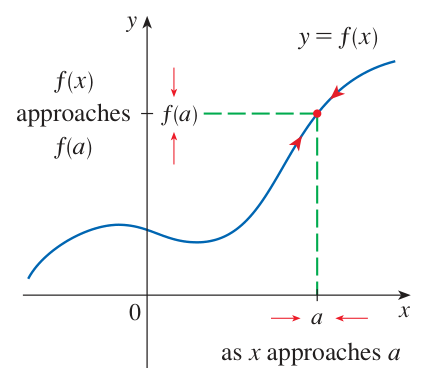
\includegraphics[width=\linewidth]{images/p0150_fig1.png}
  \vspace{1mm}
  
  {\fontsize{8.5}{10}\selectfont\textbf{\textsf{HÌNH 1}}}
  
  \vspace{16mm} % Dóng hàng Hình 2 ngang với VÍ DỤ 1
  \noindent
  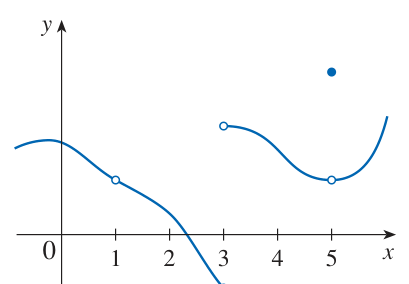
\includegraphics[width=\linewidth]{images/p0150_fig2.png}
  \vspace{1mm}
  
  {\fontsize{8.5}{10}\selectfont\textbf{\textsf{HÌNH 2}}}
\end{minipage}%
\hspace{8mm}%
\begin{minipage}[t]{124mm}
  % CỘT CHÍNH (Nội dung lý thuyết và ví dụ)
  {\fontsize{10.5}{13}\selectfont
  \textbf{\textcolor{stewartblue}{\rule{1.2ex}{1.2ex}}\hspace{0.5em}Tính liên tục của một hàm số}
  \vspace{2mm}
  
  Ở Mục~2.3, chúng ta đã nhận thấy rằng giới hạn của một hàm số khi $x$ tiến tới $a$ thường có thể tìm được đơn giản bằng cách tính giá trị của hàm số tại $a$. Các hàm số có tính chất này được gọi là \emph{liên tục tại $a$}. Chúng ta sẽ thấy rằng định nghĩa toán học về tính liên tục rất sát với ý nghĩa của từ \emph{liên tục} trong ngôn ngữ hàng ngày. (Một quá trình liên tục là một quá trình diễn ra không bị gián đoạn.)
  }
  
  \vspace{3mm}
  
  % Hộp Định nghĩa 1 viền đỏ
  \begin{tcolorbox}[
      enhanced,
      colback=white,
      colframe=defred,
      boxrule=0.75pt,
      arc=1mm,
      left=8pt, right=8pt, top=6pt, bottom=6pt
  ]
    {\bfseries\sffamily\textcolor{defred}{\fboxrule=0.75pt\fbox{\textbf{1}}\hspace{0.5em}Định nghĩa}}\hspace{0.5em}
    Hàm số $f$ được gọi là \textbf{liên tục tại một số $a$} nếu
    \[
      \lim_{x \to a} f(x) = f(a)
    \]
  \end{tcolorbox}
  
  \vspace{2mm}
  {\fontsize{9.5}{12.5}\selectfont
  Lưu ý rằng Định nghĩa~1 ngầm đòi hỏi ba điều kiện nếu $f$ liên tục tại $a$:
  
  \begin{enumerate}[label=\textbf{\arabic*.}, leftmargin=16pt, itemsep=2pt, topsep=2pt, parsep=0pt]
    \item $f(a)$ được xác định (nghĩa là, $a$ thuộc tập xác định của $f$)
    \item $\lim\limits_{x \to a} f(x)$ tồn tại
    \item $\lim\limits_{x \to a} f(x) = f(a)$
  \end{enumerate}
  
  \vspace{2mm}
  Định nghĩa nói rằng $f$ liên tục tại $a$ nếu $f(x)$ tiến tới $f(a)$ khi $x$ tiến tới $a$. Do đó, một hàm liên tục $f$ có tính chất là một sự thay đổi nhỏ của $x$ chỉ tạo ra một sự thay đổi nhỏ của $f(x)$. Trên thực tế, sự thay đổi của $f(x)$ có thể được giữ nhỏ tùy ý bằng cách giữ cho sự thay đổi của $x$ đủ nhỏ.
  
  Nếu $f$ được xác định gần $a$ (nói cách khác, $f$ được xác định trên một khoảng mở chứa $a$, ngoại trừ có thể tại $a$), ta nói rằng $f$ \textbf{gián đoạn tại $a$} (hoặc $f$ có một \textbf{điểm gián đoạn} tại $a$) nếu $f$ không liên tục tại $a$.
  
  Các hiện tượng vật lý thường diễn ra liên tục. Chẳng hạn, độ dịch chuyển hoặc vận tốc của một phương tiện đang chuyển động thay đổi liên tục theo thời gian, chiều cao của một người cũng vậy. Nhưng các điểm gián đoạn vẫn xảy ra trong những tình huống như dòng điện. [Hàm Heaviside, được giới thiệu ở Mục~2.2, gián đoạn tại $0$ vì $\lim_{t \to 0} H(t)$ không tồn tại.]
  
  Về mặt hình học, bạn có thể hình dung một hàm số liên tục tại mọi điểm trên một khoảng là một hàm có đồ thị liền nét: đồ thị có thể được vẽ mà không cần nhấc bút lên khỏi mặt giấy.
  
  \vspace{3mm}
  \textbf{\textsf{\textcolor{stewartblue}{VÍ DỤ 1}}}\hspace{0.8em}Hình~2 thể hiện đồ thị của hàm số $f$. Hàm số gián đoạn tại những điểm nào? Tại sao?
  
  \vspace{1.5mm}
  \textbf{\textsf{\textcolor{stewartblue}{LỜI GIẢI}}}\hspace{0.8em}Dường như có một điểm gián đoạn khi $a = 1$ vì đồ thị bị đứt đoạn tại đó. Lý do chính thức khiến $f$ gián đoạn tại 1 là vì $f(1)$ không được xác định.
  
  Đồ thị cũng có một điểm đứt khi $a = 3$, nhưng lý do gián đoạn thì khác. Ở đây, $f(3)$ được xác định, nhưng $\lim_{x \to 3} f(x)$ không tồn tại (vì giới hạn trái và giới hạn phải khác nhau). Do đó $f$ gián đoạn tại 3.
  
  Còn tại $a = 5$ thì sao? Ở đây, $f(5)$ được xác định và $\lim_{x \to 5} f(x)$ tồn tại (vì giới hạn trái và giới hạn phải bằng nhau). Nhưng
  \[
    \lim_{x \to 5} f(x) \neq f(5)
  \]
  Vậy $f$ gián đoạn tại 5.\hfill\textcolor{stewartblue}{\rule{1.2ex}{1.2ex}}
  
  \vspace{3mm}
  Bây giờ chúng ta hãy xem cách nhận biết các điểm gián đoạn khi một hàm số được xác định bởi một công thức.
  }
\end{minipage}
